\documentclass{article}
\usepackage{graphicx}
\usepackage{tikz}
\usepackage{pgfplots}
\usepackage{pgfplotstable}
\usepackage{filecontents}
\usepackage[T1]{fontenc}
\usepackage[utf8]{inputenc}
\usepackage[english, russian]{babel}

\renewcommand{\labelitemii}{$\circ$}

\usepackage{array}
\usepackage[table]{xcolor}
\setlength{\tabcolsep}{18pt}
\renewcommand{\arraystretch}{1.5} % Cell height scaling
\setlength{\arrayrulewidth}{0.5mm} % Table border thickness

\title{Исследование функций нервной системы на базе нейростимуляции}
\author{Нестеров И.Д., Шацких И.М., Щеглюк А.}
\date{}

\begin{document}
    \selectlanguage{russian}
    \maketitle
    \tableofcontents
    \newpage

    \addcontentsline{toc}{section}{Введение}
    \section*{Введение}

        \hspace*{4mm}\textbf{\textit{Цель работы:}} Ознакомиться с электронейромиографией на базе нейростимулятора.
        На основе стимуляций вычислить скорость распространения возбуждения. 

        \addcontentsline{toc}{subsection}{Физиология нервной системы человека}
        \subsection*{Физиология нервной системы человека}

        \hspace*{4mm} Нервная система представляет собой сеть нейронов, основной функцией
        которой является генерация, модуляция и передача информации между
        различными частями человеческого тела. Это свойство обеспечивает многие
        важные функции нервной системы, такие как регуляция жизненно важных
        функций организма (сердцебиение, дыхание, пищеварение), ощущения и
        движения тела. В конечном счете, структура нервной системы контролируют
        все физиологические и психофизиологические процессы.
        \vspace*{4mm}

        Нервная система состоит из двух отделов, связанная сетью нейронов,
        которая отправляет, получает и модулирует нервные импульсы между
        различными частями тела:

        \begin{itemize}
            \item \textit{Центральная нервная система} (ЦНС) является интеграционным и
            командным центром организма.

            \item \textit{Периферическая нервная система} (ПНС) представляет собой канал
            между ЦНС и организмом. Далее она подразделяется на \textit{соматическую
            нервную систему} (СНС) и \textit{вегетативную нервную систему} (ВНС).
        \end{itemize}

        В нервной системе присутствуют два основных типа клеток – это нейроны
        и глиальные клетки.
        \vspace*{4mm}

        Нейроны, или нервные клетки, являются основными структурными и
        функциональными единицами нервной системы (рис. 1). Каждый нейрон
        состоит из тела (\textit{сомы}) и ряда отростков (\textit{нейритов}). Тело нервной клетки
        содержит клеточные органеллы и является местом генерации нервных импульсов
        (\textit{потенциалов действия}). Процессы исходят из организма, они соединяют
        нейроны друг с другом и с другими клетками тела, обеспечивая поток нервных
        импульсов. Существует два типа нервных процессов, которые различаются по
        структуре и функциям:

        \begin{itemize}
            \item \textit{Аксоны} длинные и проводят импульсы от тела нейрона.

            \item \textit{Дендриты} короткие и принимают импульсы от других нейронов,
            проводя электрический сигнал к телу нервной клетки.
        \end{itemize}
        \newpage
        
        \begin{figure}[t]
            \centering
            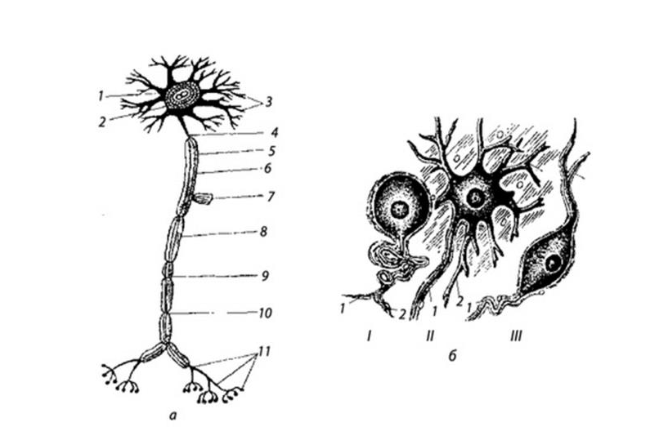
\includegraphics[width=\textwidth]{data/Нейрон.png}
            \caption{Схема нейрона (по И.Ф. Иванову): 1 - тело; 2 - ядро; 3 - дендриты;
            4,6 - нейриты; 5,8 - миелиновая оболочка; 7 - коллатераль; 9 - перехват/узел Ранвье;
            10 - ядро леммоцита; 11 - нервные окончания; I - униполярная; II - мультаполярная;
            III - биполярная; 1 - неврит; 2 - дендрит.}
        \end{figure}

        Каждый нейрон имеет один аксон, а количество дендритов варьируется.
        Исходя из этого числа, существует четыре структурных типа нейронов:
        \textit{мультиполярный}, \textit{биполярный}, \textit{псевдоуниполярный} и \textit{униполярный}.
        \vspace*{4mm}

        Существует два типа нейронов, названных в зависимости от того,
        посылают ли они электрический сигнал в сторону ЦНС или от нее:

        \begin{itemize}
            \item \textit{Эфферентные нейроны} (моторные или нисходящие) посылают нервные
            импульсы от ЦНС к периферическим тканям, инструктируя их, как
            функционировать.

            \item \textit{Афферентные нейроны} (сенсорные или восходящие) проводят
            импульсы от периферических тканей к ЦНС. Эти импульсы содержат
            сенсорную информацию, описывающую среду ткани.
        \end{itemize}

        Место, где аксон соединяется с другой клеткой для передачи нервного
        импульса, называется синапсом (рис. 2). Синапс не соединяется напрямую со
        следующей клеткой. Вместо этого импульс вызывает выброс химических
        веществ, называемых нейротрансмиттерами, из самого конца аксона. Эти
        нейротрансмиттеры связываются с мембраной эффекторной клетки, вызывая
        биохимические события, происходящие внутри этой клетки в соответствии с
        приказами, посылаемыми ЦНС.
        \newpage

        \begin{figure}[t]
            \centering
            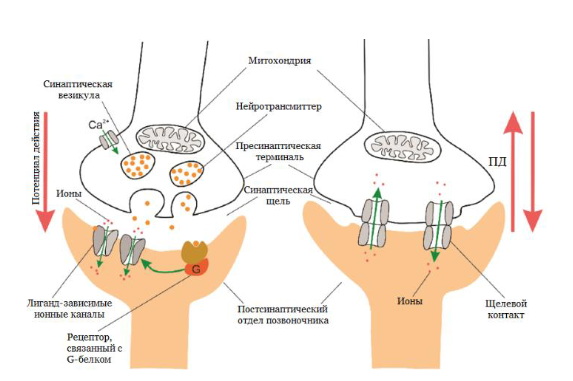
\includegraphics[width=\textwidth]{data/Синапс.png}
            \caption{Структура синапса.}
        \end{figure}

        \textit{Синапс} – это функциональное соединение между нервным волокном и
        иннервируемой тканью. Синапс обеспечивает передачу возбуждения от нервного
        волокна к иннервируемой им ткани – мышечной, нервной или железистой.
        \vspace*{4mm}

        Каждое разветвление аксона заканчивается аксон-терминальной
        выпуклостью, похожей на луковицу, это синаптическая пуговка, которая
        располагается в углублении сарколеммы. Эта часть сарколеммы называется
        концевой пластинкой. Если нервное волокно иннервирует мышечную ткань,
        синапс называется \textit{нервно-мышечным}.
        \vspace*{4mm}

        \textit{Глиальные клетки}, также называемые нейроглией или просто глией,
        представляют собой более мелкие невозбуждающие клетки, которые
        поддерживают нейроны. Они не распространяют потенциалы действия. Вместо
        этого они миелинизируют нейроны, поддерживают гомеостатический баланс,
        обеспечивают структурную поддержку, защиту и питание нейронов во всей
        нервной системе.
        \newpage

        Этот набор функций обеспечивают четыре разных типа глиальных клеток:

        \begin{itemize}
            \item Миелинизирующая глия образует миелиновую оболочку, изолирующую
            аксоны. Они называются \textit{олигодендроцитами} в ЦНС и \textit{шванновскими
            клетками} в ПНС.

            \item \textit{Астроциты} (ЦНС) и \textit{сателлитные глиальные клетки} (ПНС) выполняют
            общую функцию поддержки и защиты нейронов.

            \item Два других типа глиальных клеток встречаются исключительно в ЦНС:
                \begin{itemize}
                    \item \textit{Микроглия} — это фагоциты ЦНС.
                    \item \textit{Эпендимальные клетки}, выстилающие желудочковую систему ЦНС.
                \end{itemize} 
        \end{itemize}

        Большинство аксонов покрыто белым изолирующим веществом,
        называемым \textit{миелиновой оболочкой}, которое вырабатывается
        олигодендроцитами и шванновскими клетками. Миелин сегментарно
        окружает аксон, оставляя безмиелиновые промежутки между сегментами,
        называемые перехватами Ранвье (рис. 3). Нейронные импульсы
        распространяются только через узлы Ранвье, минуя миелиновую оболочку. Это
        значительно увеличивает скорость распространения нервного импульса.

        \begin{figure}[h]
            \centering
            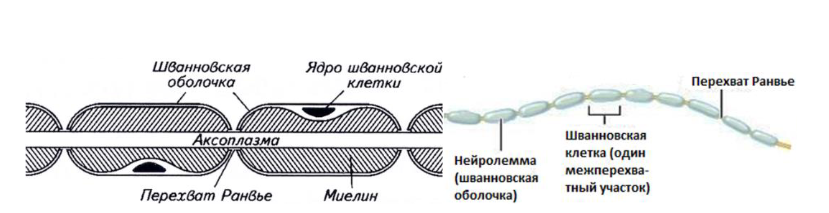
\includegraphics[width=\textwidth]{data/Глиальная клетка.png}
            \caption{Пример структуры глиальной клетки.}
        \end{figure}

        За счет милеинового слоя можно выделить два типа проведения сигнала по
        нерву – сальтаторное и непрерывное.
        \vspace*{4mm}

        \textit{Сальтаторная проводимость} происходит в миелинизированных аксонах,
        которые позволяют потенциалу действия возникать только в перехватах Ранвье.
        Следовательно, нервные импульсы распространяются быстро, прыгая от одного
        узла Ранвье к следующему узлу. Поэтому сальтаторное проводимость — самый
        быстрый способ передачи потенциала действия. Напротив, непрерывная
        проводимость имеет место в немиелинизированных аксонах. Потенциал
        действия генерируется по всей длине немиелинизированного аксона.
        Следовательно, он передает нервные импульсы медленно. Кроме того,
        сальтаторное проведение более эффективно, поскольку его энергетические
        затраты невелики по сравнению с продолжительным проведением.
        \newpage

        \addcontentsline{toc}{subsection}{Передача информации в нервной системе}
        \subsection*{Передача информации в нервной системе}

        \hspace*{4mm} Раньше нервное волокно и его содержимое сравнивали с металлической
        проволокой, а мембрану — с изоляцией вокруг провода. Это сравнение было
        ошибочным по ряду причин. Носителями заряда в нервах являются ионы, а не
        электроны, и плотность ионов в аксоне значительно меньше, чем электронов в
        металлической проволоке. Например, в реакции образования соли из натрия и
        хлора каждый атом натрия отдает отрицательно заряженный электрон атому
        хлора. В результате получается хлорид натрия (NaCl), состоящий из одного
        положительно заряженного иона натрия (Na+) и одного отрицательно
        заряженного иона хлорида (Cl–). Положительно заряженный ион называется
        \textit{катионом}; отрицательно заряженный ион - \textit{анионом}. Электрические события,
        составляющие передачу сигналов в нервной системе, зависят от распределения
        таких ионов по обе стороны нервной мембраны.
        \vspace*{4mm}

        Электрический потенциал, существующий в нейронах, основан на
        распределении ионов через плазматическую мембрану и что это распределение
        происходит за счет проникновения через мембрану. Фактически ионы почти
        всегда гидратированы в виде ионно-водных комплексов, которые с большим
        трудом проникают через гидрофобный липидный бислой плазматической
        мембраны. Проникновение фактически происходит через встроенные в него
        белковые структуры в липидном бислое и охватывает мембрану от цитоплазмы
        до внеклеточной жидкости.
        \vspace*{4mm}

        Нейрон находится в состоянии покоя, когда он не посылает электрический
        сигнал. В это время внутренняя часть нейрона отрицательна по отношению к
        внешней. Хотя концентрации различных ионов пытаются сбалансироваться по
        обе стороны мембраны, это не удается, поскольку клеточная мембрана позволяет
        только некоторым ионам проходить через ионные каналы. В состоянии
        покоя ионы калия (K+) легко проникают через мембрану. Также в состоянии покоя
        ионам хлорида (Cl–) и ионам натрия (Na+) труднее проникать. Потенциал покоя
        нейрона составляет около -70 мВ – это означает, что внутри нейрона на 70 мВ
        меньше, чем снаружи (рис. 4).
        \newpage

        \begin{figure}[t]
            \centering
            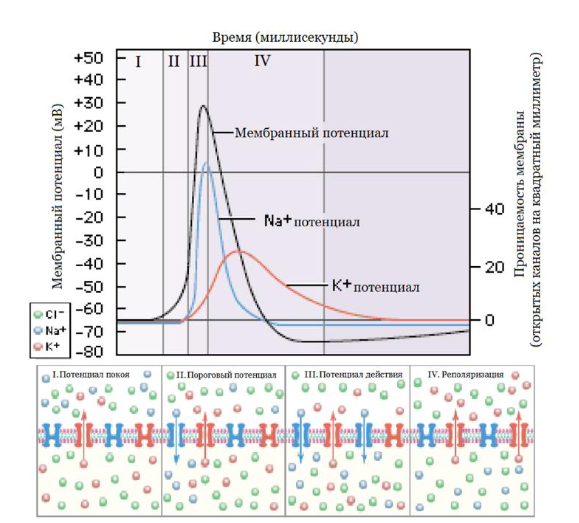
\includegraphics[width=\textwidth]{data/Потенциал действия.png}
            \caption{Графическая зависимость ионной проницаемости и потенциала действия.}
        \end{figure}

        Потенциал действия возникает, когда нейрон отправляет информацию по
        аксону в сторону от тела клетки. \textit{Потенциал действия} – это вспышка электрической
        активности, создаваемый деполяризующим током. Это означает, что какое-то
        событие (стимул) заставляет потенциал покоя двигаться в сторону 0 мВ. Когда
        деполяризация достигает примерно -55 мВ, нейрон запускает потенциал действия.
        \newpage

    \addcontentsline{toc}{section}{Ход работы}
    \section*{Ход работы}

        \addcontentsline{toc}{subsection}{Оборудование}
        \subsection*{Оборудование}

            \hspace*{4mm} В ходе лабораторной работы использовался нейростимулятор. Он состоял из регистрирующего
            и стимулирующего электродов. Также вспомогательно использовались спиртосодержащие салфетки
            для очистки электродов и нивелирования жировых выделений, увеличивающих импеданс, а также 
            электролитный гель.

        \addcontentsline{toc}{subsection}{Методы и результаты}
        \subsection*{Методы и результаты}

            \hspace*{4mm} Во время проведения эксперимента регистрирующий электрод располагался на фаланге среднего пальца правой руки.
            Стимуляция производилась последовательно в трёх местах: запястье (рис. 5), локтевой сгиб (рис. 6) и нижняя треть плеча (рис. 7).

            \begin{figure}[h]
                \centering
                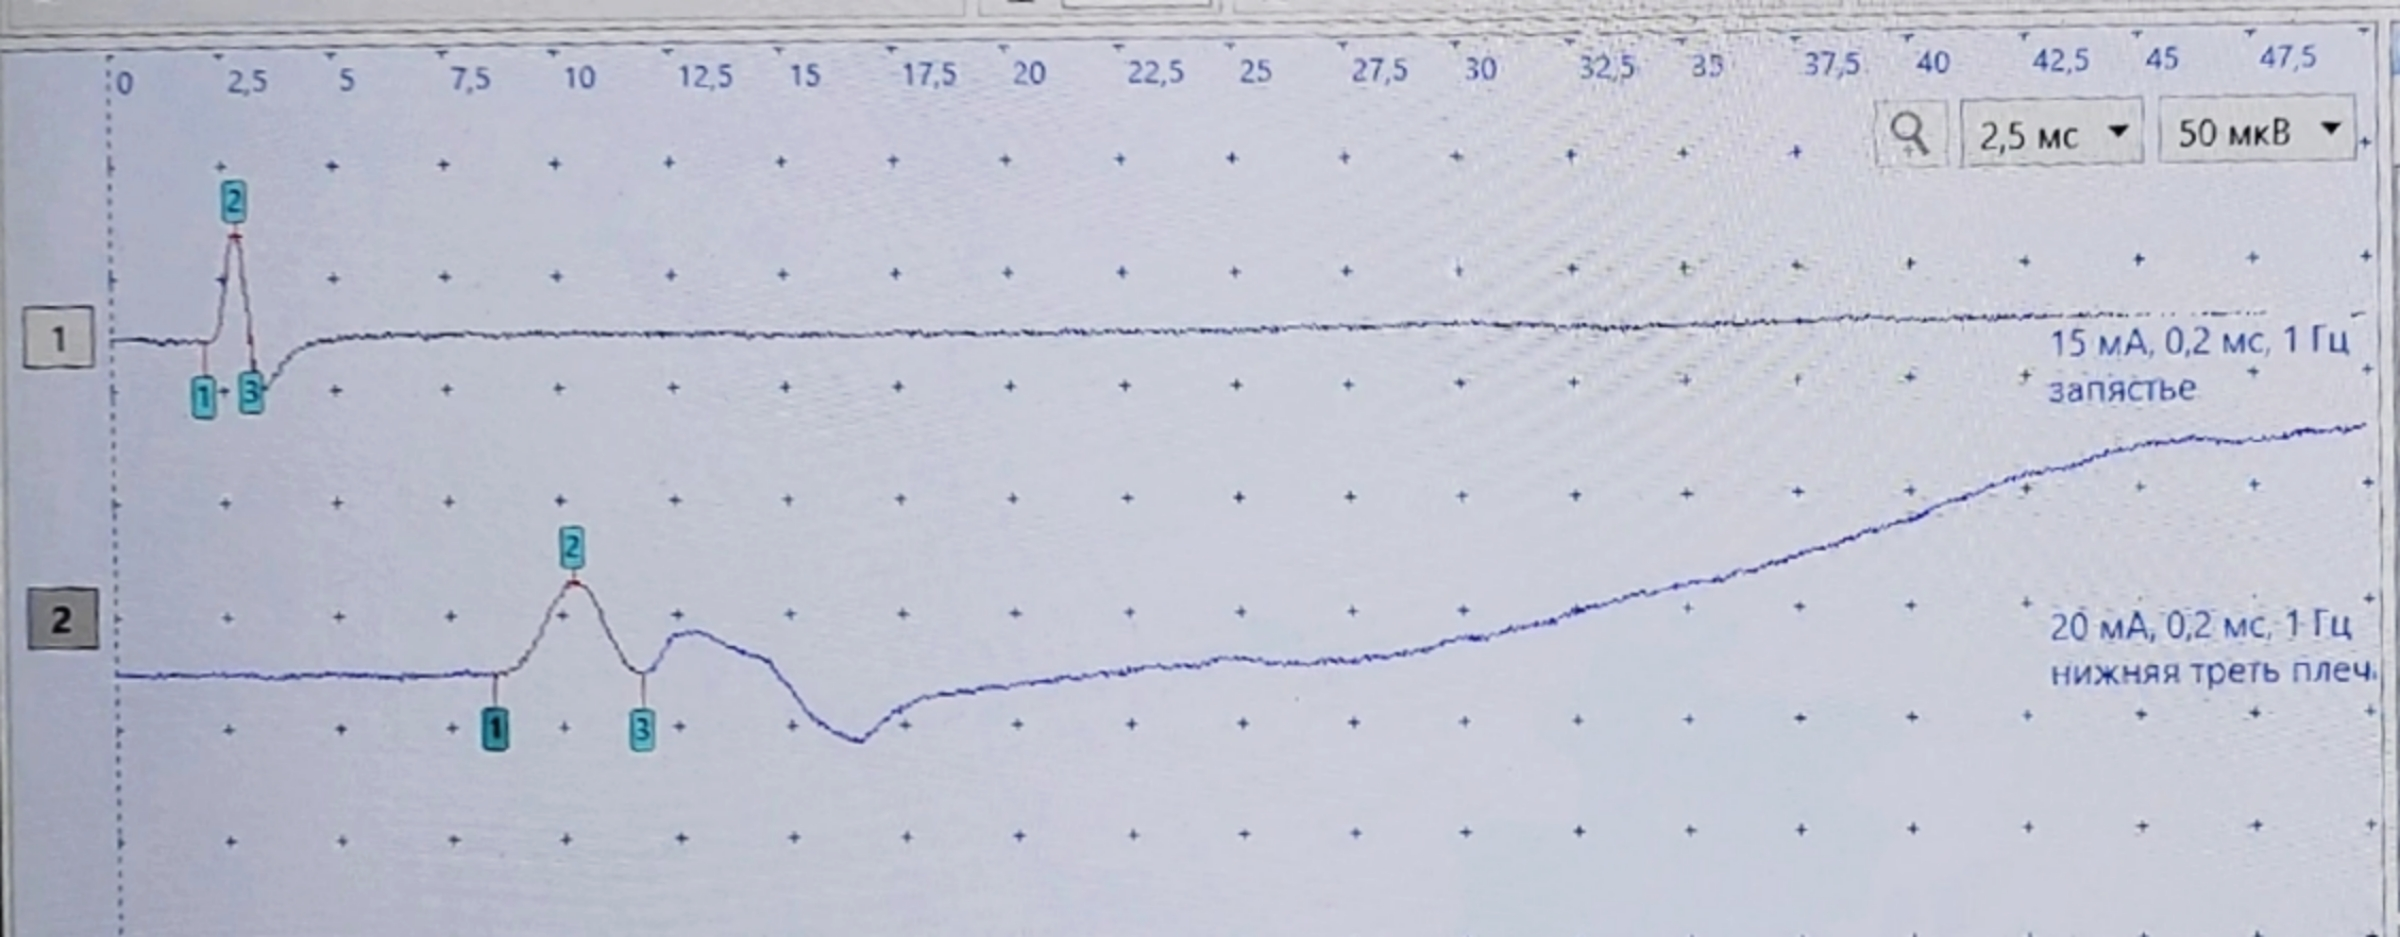
\includegraphics[width=\textwidth]{data/1,2.jpg}
                \caption{Ответный сигнал на стимуляцию запястья (Сверху).}
            \end{figure}

            \begin{center}
                Параметры стимуляции:    
            \end{center}
            
            \begin{center}
                \begin{tabular}{|l|l|}
                    \hline
                    Точка стимуляции & Запястье \\ \hline
                    Латентность, мс & 2.0 \\ \hline
                    Расстояние, мм & 135 \\ \hline
                    Амплитуда, мВ & 0.05 \\ \hline
                    Длительность, мс & 1.1  \\ \hline
                \end{tabular}
            \end{center}
            \newpage

            \begin{figure}[h]
                \centering
                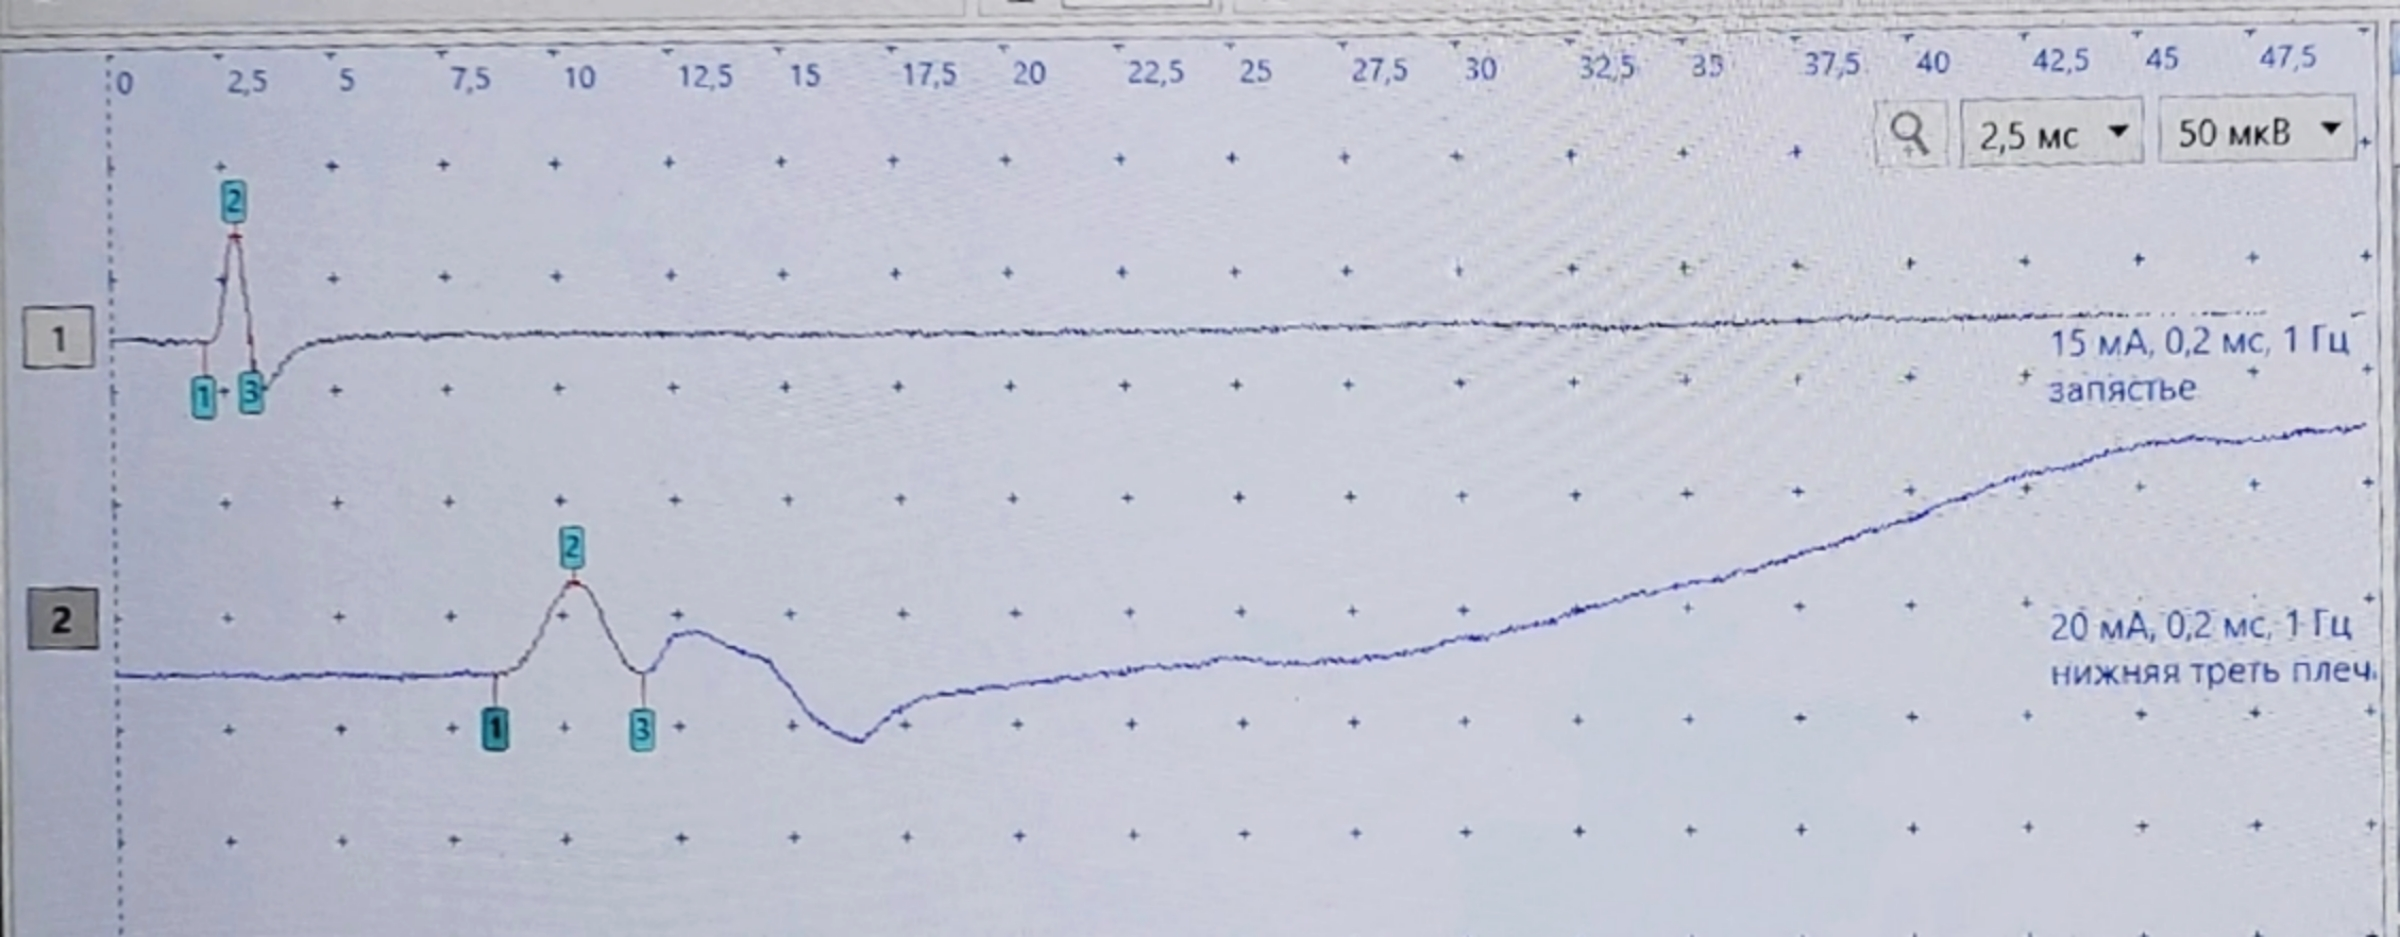
\includegraphics[width=\textwidth]{data/1,2.jpg}
                \caption{Ответный сигнал на стимуляцию нижней трети плеча (Снизу).}
            \end{figure}

            \begin{center}
                Параметры стимуляции:    
            \end{center}

            \begin{center}
                \begin{tabular}{|l|l|}
                    \hline
                    Точка стимуляции & Нижняя треть плеча \\ \hline
                    Латентность, мс & 8.4 \\ \hline
                    Расстояние, мм & 70 \\ \hline
                    Амплитуда, мВ & 0.04 \\ \hline
                    Длительность, мс & 3.3  \\ \hline
                \end{tabular}
            \end{center}
            \newpage

            \begin{figure}[h]
                \centering
                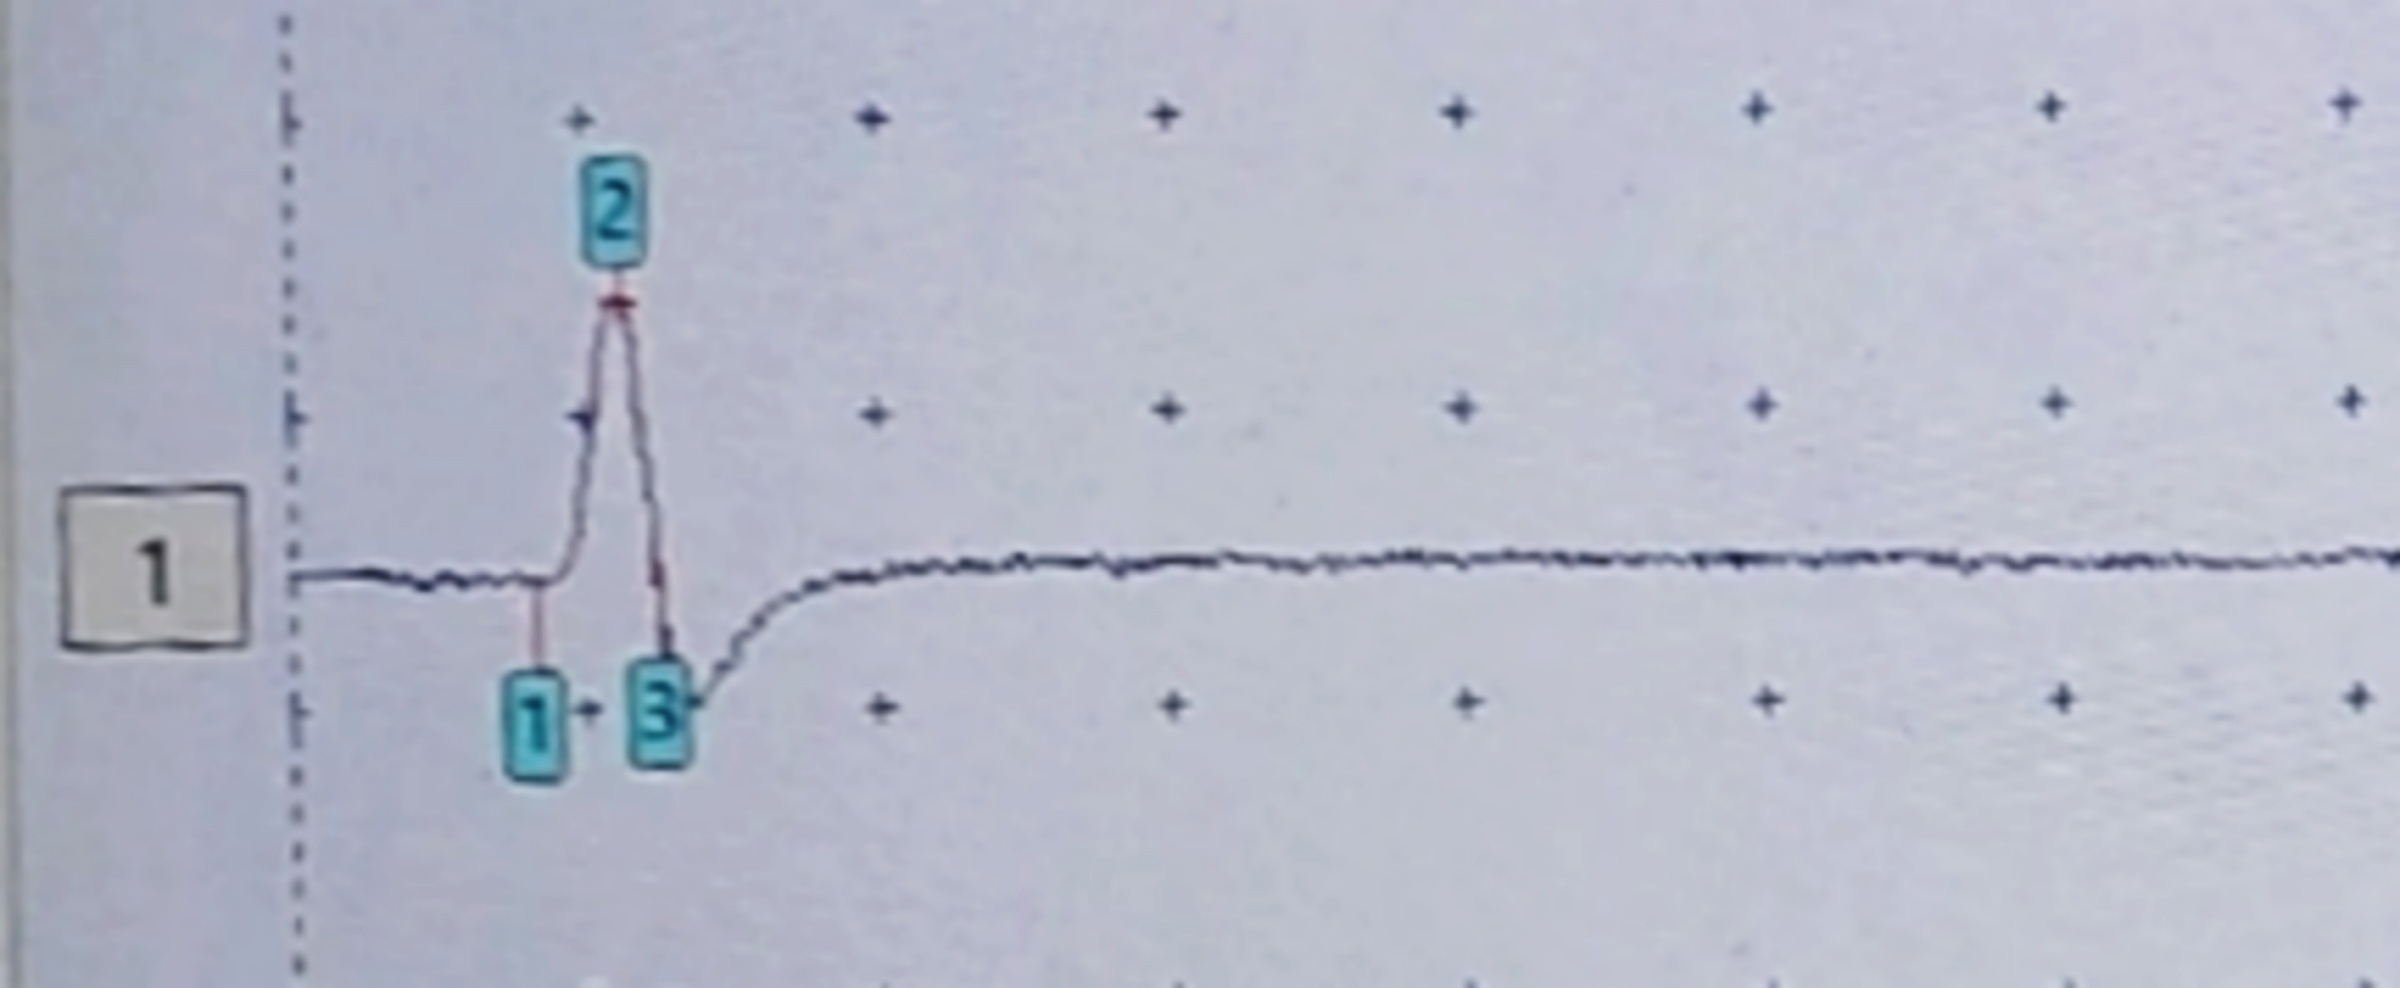
\includegraphics[width=\textwidth]{data/3.jpg}
                \caption{Ответный сигнал на стимуляцию локтевого сгиба.}
            \end{figure}

            \begin{center}
                Параметры стимуляции:    
            \end{center}

            \begin{center}
                \begin{tabular}{|l|l|}
                    \hline
                    Точка стимуляции & Локтевой сгиб \\ \hline
                    Латентность, мс & 5.2 \\ \hline
                    Расстояние, мм & 233 \\ \hline
                    Амплитуда, мВ & 0.02 \\ \hline
                    Длительность, мс & 1.6  \\ \hline
                \end{tabular}
            \end{center}
            
                \addcontentsline{toc}{subsubsection}{Вычисление СРВ}
                \subsubsection*{Вычисление СРВ}

                    \hspace*{4mm} При помощи полученных данных может быть вычислена \textit{скорость распространения возбуждения} (СРВ):

                    \begin{equation}
                        CPB = \frac{D_{P} - D_{D}}{T_{P} - T_{D}}
                    \end{equation}

                    Где $D_{P} - D_{D}$ - разность длин между проксильмальной и дистальной точками стимуляции относительно
                    регистрирующего электрода. $T_{P} - T_{D}$ - разность латентностей при стимуляции проксильмальной и
                    дистальной точек соответственно.

                    Найдём 3 величины СРВ:

                    \begin{itemize}
                        \item СРВ{з-л} - между запястьем и локтевым сгибом.
                        \item СРВ{л-п} - между локтевым сгибом и нижней третью плеча.
                        \item СРВ{з-п} - между запястьем и нижней третью плеча.
                    \end{itemize}
                    \newpage

                    После подстановки значений получаем результаты:

                    \begin{itemize}
                        \item СРВ{з-л} $\approx$ 30 м/с.
                        \item СРВ{л-п} $\approx$ 10 м/с.
                        \item СРВ{з-п} $\approx$ 48 м/с.
                    \end{itemize}

                    Порядок величин совпадает с истинными значениями.

    \addcontentsline{toc}{section}{Выводы}
    \section*{Выводы}

        \hspace*{4mm} В данной работе был проведён ряд стимуляций нейро-мышечного волокна. С помощью параметров
        ответных сигналов были вычислены скорости распространения возбуждения волокна в разных частях руки, которые
        согласуются с известными результатами.










\end{document}